\documentclass[12pt,openany,a4paper]{book}
\usepackage{graphicx}	% if you want encapsulated PS figures.
\usepackage{cite}
\usepackage{listings}
\usepackage{pgfgantt}
\usepackage{amsmath}
\usepackage{algorithm}
\usepackage[noend]{algpseudocode}
\usepackage{float}
\usepackage{xcolor}
\usepackage{tikz}
\graphicspath{{../demo_pictures/pngs/}}

% If you use a macro file called macros.tex :
% \input{macros}
% Note: The present document has its macros built in.

% Number subsections but not subsubsections:
\setcounter{secnumdepth}{2}
% Show subsections but not subsubsections in table of contents:
\setcounter{tocdepth}{2}

\pagestyle{headings}		% Chapter on left page, Section on right.
\raggedbottom

\setlength{\topmargin}		{-5mm}  %  25-5 = 20mm
\setlength{\oddsidemargin}	{10mm}  % rhs page inner margin = 25+10mm
\setlength{\evensidemargin}	{0mm}   % lhs page outer margin = 25mm
\setlength{\textwidth}		{150mm} % 35 + 150 + 25 = 210mm
\setlength{\textheight}		{240mm} % 

\renewcommand{\baselinestretch}{1.2}	% Looks like 1.5 spacing.

% Stop figure/tables smaller than 3/4 page from appearing alone on a page:
\renewcommand{\textfraction}{0.25}
\renewcommand{\topfraction}{0.75}
\renewcommand{\bottomfraction}{0.75}
\renewcommand{\floatpagefraction}{0.75}

% THEOREM-LIKE ENVIRONMENTS:
\newtheorem{defn}	{Definition}	% cf. \dfn for cross-referencing
\newtheorem{theorem}	{Theorem}	% cf. \thrm for cross-referencing
\newtheorem{lemma}	{Lemma}		% cf. \lem for cross-referencing

% AIDS TO CROSS-REFERENCING (All take a label as argument):
\newcommand{\eref}[1] {(\ref{#1})}		% (...)
\newcommand{\eq}[1]   {Eq.\,(\ref{#1})}		% Eq.~(...)
\newcommand{\eqs}[2]  {Eqs.~(\ref{#1}) and~(\ref{#2})}
\newcommand{\dfn}[1]  {Definition~\ref{#1}}	% Definition~...
\newcommand{\thrm}[1] {Theorem~\ref{#1}}	% Theorem~...
\newcommand{\lem}[1]  {Lemma~\ref{#1}}		% Lemma~...
\newcommand{\fig}[1]  {Fig.\,\ref{#1}}		% Fig.~...
\newcommand{\tab}[1]  {Table~\ref{#1}}		% Table~...
\newcommand{\chap}[1] {Chapter~\ref{#1}}	% Chapter~...
\newcommand{\secn}[1] {Section~\ref{#1}}	% Section~...
\newcommand{\ssec}[1] {Subsection~\ref{#1}}	% Subsection~...
\newcommand{\alg}[1]  {Algorithm~\ref{#1}}  % Algorithm~ ...
\newcommand{\app}[1]  {Appendix~\ref{#1}}   % Appendix~ ...

% AIDS TO FORMATTING:
\newcommand{\teq}[1]	{\mbox{$#1$}}	% in-Text EQuation (unbreakable)
\newcommand{\qed}	{\hspace*{\fill}$\bullet$}	% end of proof

% MATHEMATICAL TEMPLATES:
% Text or math mode:
\newcommand{\half}	{\ensuremath{\frac{1}{2}}}	% one-half
\newcommand{\halftxt}	{\mbox{$\frac{1}{2}$}}	  	% one-half, small
% Math mode only:
% N.B. Parentheses are ROUND; brackets are SQUARE!
\newcommand{\oneon}[1]	{\frac{1}{#1}}		  % reciprocal
\newcommand{\pow}[2]	{\left({#1}\right)^{#2}}  % Parenthesized pOWer
\newcommand{\bow}[2]	{\left[{#1}\right]^{#2}}  % Bracketed pOWer
\newcommand{\evalat}[2]	{\left.{#1}\right|_{#2}}  % EVALuated AT with bar
\newcommand{\bevalat}[2]{\left[{#1}\right]_{#2}}  % Bracketed EVALuated AT
% Total derivatives:
\newcommand{\sdd}[2]	{\frac{d{#1}}{d{#2}}}		    % Short
\newcommand{\sqdd}[2]	{\frac{d^2{#1}}{d{#2}^2}}	    % 2nd ("SQuared")
\newcommand{\ldd}[2]	{\frac{d}{d{#1}}\left({#2}\right)}  % Long paren'ed
\newcommand{\bdd}[2]	{\frac{d}{d{#2}}\left[{#2}\right]}  % long Bracketed
% Partial derivatives (same sequence as for total derivatives):
\newcommand{\sdada}[2]	{\frac{\partial {#1}}{\partial {#2}}}
\newcommand{\sqdada}[2]	{\frac{\partial ^{2}{#1}}{\partial {#2}^{2}}}
\newcommand{\ldada}[2]	{\frac{\partial}{\partial {#1}}\left({#2}\right)}
\newcommand{\bdada}[2]	{\frac{\partial}{\partial {#1}}\left[{#2}\right]}
\newcommand{\da}	{\partial}

% ORDINAL NUMBERS:
\newcommand{\ith}	{\ensuremath{i^{\rm th}}}
\newcommand{\jth}	{\ensuremath{j^{\rm th}}}
\newcommand{\kth}	{\ensuremath{k^{\rm th}}}
\newcommand{\lth}	{\ensuremath{l^{\rm th}}}
\newcommand{\mth}	{\ensuremath{m^{\rm th}}}
\newcommand{\nth}	{\ensuremath{n^{\rm th}}}

% SINUSOIDAL TIME AND SPACE-DEPENDENCY FACTORS:
\newcommand{\ejot}	{\ensuremath{e^{j\omega t}}}
\newcommand{\emjot}	{\ensuremath{e^{-j\omega t}}}

% UNITS (TEXT OR MATH MODE, WITH LEADING PADDING SPACE IF APPLICABLE):
% NB: These have not been tested since being modified for LaTeX2e.
\newcommand{\pack}	{\hspace{-0.08em}}
\newcommand{\Pack}	{\hspace{-0.12em}}
\newcommand{\mA}	{\ensuremath{\rm\,m\pack A}}
\newcommand{\dB}	{\ensuremath{\rm\,d\pack B}}
\newcommand{\dBm}	{\ensuremath{\rm\,d\pack B\pack m}}
\newcommand{\dBW}	{\ensuremath{\rm\,d\pack B\Pack W}}
\newcommand{\uF}	{\ensuremath{\rm\,\mu\pack F}}
\newcommand{\pF}	{\ensuremath{\rm\,p\pack F}}
\newcommand{\nF}	{\ensuremath{\rm\,n\pack F}}
\newcommand{\uH}	{\ensuremath{\rm\,\mu\pack H}}
\newcommand{\mH}	{\ensuremath{\rm\,m\pack H}}
\newcommand{\Hz}	{\ensuremath{\rm\,H\pack z}}
\newcommand{\kHz}	{\ensuremath{\rm\,k\pack H\pack z}}
\newcommand{\MHz}	{\ensuremath{\rm\,M\pack H\pack z}}
\newcommand{\GHz}	{\ensuremath{\rm\,G\pack H\pack z}}
\newcommand{\J}		{\ensuremath{\rm\,J}}
\newcommand{\kg}	{\ensuremath{\rm\,k\pack g}}
\newcommand{\K}		{\ensuremath{\rm\,K}}
\newcommand{\m}		{\ensuremath{\rm\,m}}
\newcommand{\cm}	{\ensuremath{\rm\,cm}}
\newcommand{\km}	{\ensuremath{\rm\,k\pack m}}
\newcommand{\mm}	{\ensuremath{\rm\,m\pack m}}
\newcommand{\nm}	{\ensuremath{\rm\,n\pack m}}
\newcommand{\um}	{\ensuremath{\rm\,\mu m}}
\newcommand{\Np}	{\ensuremath{\rm\,N\pack p}}
\newcommand{\s}		{\ensuremath{\rm\,s}}
\newcommand{\ms}	{\ensuremath{\rm\,m\pack s}}
\newcommand{\us}	{\ensuremath{\rm\,\mu s}}
\newcommand{\V}		{\ensuremath{\rm\,V}}
\newcommand{\mV}	{\ensuremath{\rm\,m\Pack V}}
\newcommand{\W}		{\ensuremath{\rm\,W}}
\newcommand{\mW}	{\ensuremath{\rm\,m\Pack W}}
\newcommand{\ohm}	{\ensuremath{\rm\,\Omega}}
\newcommand{\kohm}	{\ensuremath{\rm\,k\Omega}}
\newcommand{\Mohm}	{\ensuremath{\rm\,M\Omega}}
\newcommand{\degs}	{\ensuremath{\rm^{\circ}}}

\definecolor{codegreen}{rgb}{0, 0.6, 0}
\definecolor{codegrey}{rgb}{0.5, 0.5, 0.5}
\definecolor{codepurple}{rgb}{0.58, 0, 0.82}
\definecolor{backcolour}{rgb}{0.95, 0.95, 0.92}

\lstdefinestyle{codestyle}{
    backgroundcolor=\color{backcolour},
    commentstyle=\color{codegreen},
    keywordstyle=\color{magenta},
    numberstyle=\tiny\color{codegrey},
    stringstyle=\color{codepurple},
    basicstyle=\ttfamily\footnotesize,
    breakatwhitespace=false,
    breaklines=true,
    captionpos=b,
    keepspaces=true,
    numbers=left,
    numbersep=5pt,
    showspaces=false,
    showstringspaces=false,
    showtabs=false,
    tabsize=4
}

\renewcommand{\lstlistingname}{Code Snippet}
\renewcommand{\lstlistlistingname}{List of Code Snippets}

% LaTeX run-time type-in command:
%
\typein{Enter \protect\includeonly{...} command (or just type RETURN):}
%
% Uncommenting this command makes LaTeX prompt you for the \includeonly
% list.  At the prompt
%
%	\@typein=
%
% you type
%
%	\includeonly{chap1,chap2}
%
% to include the files chap1.tex and chap2.tex and omit any others.
% To include every \include file, just hit RETURN.
% If you are running LaTeX from xtexsh, you may need to click the mouse
% in the LaTeX window to position the cursor at the \@typein prompt.

\begin{document}

\frontmatter
% By default, frontmatter has Roman page-numbering (i,ii,...).

\begin{titlepage}
\begin{center}
\includegraphics[width=\linewidth]{UQLogo.png}
\end{center}
\renewcommand{\baselinestretch}{1.0}
\begin{center}
\vspace*{35mm}
\Huge\bf
        Investigating A Linear\\
        Approach to Arithmetic\\
        Re-Association within GraalVM\\
\vspace{20mm}
\large\sl
		by\\
		Nathan Corcoran
		\medskip\\
\rm
		School of Electrical Engineering and Computer Science,\\
		The University of Queensland.\\
\vspace{30mm}
		Submitted for the degree of\\
		Bachelor of Engineering
		\smallskip\\
\normalsize
		in the field of Software Engineering
		\medskip\\
\large
		November 2024.
\end{center}
\end{titlepage}

\cleardoublepage

\begin{flushright}
    Nathan Corcoran\\
    n.corcoran@uq.edu.au\\
	\medskip
	\today
\end{flushright}
\begin{flushleft}
  Prof Michael Bruenig\\
  Head of School\\
  School of Electrical Engineering and Computer Science\\
  The University of Queensland\\
  St Lucia, QLD 4072\\
  \bigskip\bigskip
  Dear Professor Bruenig,
\end{flushleft}

In accordance with the requirements of the degree of Bachelor of
Engineering in the division of 
Software Engineering,
I present the
following thesis entitled ``Investigating A Linear Approach
to Arithmetic Re-Association within GraalVM''.  
This work was performed under the supervision of
A/Prof.\ Mark Utting, Prof.\ Ian J.\ Hayes and, Mr.\ Brae Webb.

I declare that the work submitted in this thesis is my own, except as
acknowledged in the text and footnotes, and has not been previously
submitted for a degree at The University of Queensland or any other
institution.

\begin{flushright}
	Yours sincerely,\\
	\medskip
    \includegraphics[width=0.3\linewidth]{my_signature}\\
	\medskip
	Nathan Corcoran.
\end{flushright}

\cleardoublepage

\chapter{Acknowledgments}

I would like to acknowledge my supervisors A/Prof.\ Mark Utting, Prof.\ Ian J.\
Hayes, and Mr.\ Brae Webb for their continual support and guidance throughout
the entire project. Thank you all for enabling me to learn a great deal through 
this experience.

\cleardoublepage

\chapter{Abstract}

Optimising compilers are essential tools for building efficient modern
programs. The GraalVM compiler, released by Oracle,
aims to achieve high levels of optimisation. Arithmetic expressions provide
many opportunities for optimisation, with arithmetic re-association playing
a crucial role in identifying chances for further optimisations. Currently,
when re-associating complex expressions, the GraalVM compiler's method
of graph manipulations are insufficient. By reducing arithmetic 
expressions to a list of operands, they can be ranked common factors and through
a simple sort like-terms can be grouped. From this, algebraic simplifications can
be as trivial as removing elements within the list. This approach simplifies the re-association
process and allows the GraalVM compiler to apply further optimisations that
were not previously identifiable.

\tableofcontents

\listoffigures
\addcontentsline{toc}{chapter}{List of Figures}

\lstlistoflistings
\addcontentsline{toc}{chapter}{List of Code Snippets}

% If file los.tex begins with ``\chapter{List of Symbols}'':
% \include{los}

\cleardoublepage

\mainmatter
% By default, mainmatter has Arabic page-numbering (1,2,...).


% Chapters may be \include files, each beginning with a line like
%
%	\chapter{Title of chapter}
%
% e.g. if two chapter files were called intro.tex and theory.tex,
% we would say
%
%	\include{intro}
%	\include{theory}

\chapter{Introduction}
\label{intro}

Optimising compilers are a crucial tool for building efficient 
modern programs. They allow developers to write highly abstracted code without 
sacrificing program performance. High-level abstractions are relied upon when
programming complex models that many of modern software requires. The GraalVM
compiler, released by Oracle, is one such compiler that aims to achieve 
high-levels of optimisation. Arithmetic expressions allow for many optimisation opportunities.
Arithmetic re-association plays a pivotal role in this. The method is not used
to optimise the code by itself, but rather to create opportunities for further
optimisations. Consequently, to maximise the effectiveness of an optimising
compiler, we must ensure effectiveness of re-association methods. That is,
expressions need to be represented in such a way that eases the implementation
of optimisations.
Currently, the GraalVM compiler optimises expressions by way 
of graph comparisons and manipulations invoked via the \verb|ReassociationPhase|~\cite{graalsrc}.
This phase, for example, would take an expression such as \verb|x + y + z - z - y| and
re-order its sub-expressions such that like-terms are grouped, possibly forming
\verb|x - x + y - y + z|. The compiler can then non-trivially apply, in this
instance, algebraic simplifications to produce just \verb|z|.
For complex expressions, the GraalVM compiler's approach to re-association are inexhaustive
and potentially computationally expensive. By replacing the current method with 
our list-based approach, arithmetic re-association is trivial. \\
In this report, a method of arithmetic re-association is proposed that re-orders
expressions by manipulating a list of its operands. It will be shown that by
ranking and sorting a list of operands, further expression optimisations
can be identified and applied by the GraalVM compiler. \\
\chap{bg} covers background information regarding arithmetic re-association;
some common algebraic simplifications; the role of intermediate representation
within compiler design, detailing how arithmetic expressions can be represented;
and finally the GraalVM compiler itself. \\
\chap{litrev} investigates known methods of arithmetic re-association and 
a method of testing optimising compilers. \\
\chap{methods} details the proposed list-based approach, covering the steps
of graph preparation, expression tree flattening, operand ranking, a possible 
method of optimising certain expression trees, and expression tree 
reconstruction. Testing performed and problems that
arose during the implementation process are also included. \\
\chap{results} shows and discusses that the proposed approach successfully
re-associates and simplifies complex arithmetic expressions. \\
\chap{conclusion} summarises this report and presents possible further work for 
future researchers.

\chapter{Background}
\label{bg}

\section{Arithmetic Re-Association}
\label{ara}

Arithmetic re-association utilises the associative and
commutative properties of certain arithmetic operators to re-arrange expressions~\cite{redund}. 
This may allow simplifications that were not easily identified in the original 
expression to be made evident. Re-association methods use associative,
distributive, and commutative properties of some operators to re-order arithmetic
expressions.
Using re-association, a compiler would transform the expression
\verb|x = 23 + i + y + 43 + i| into the form \\ \verb|x = i + i + y + 23 + 43|. It
is now easier for the compiler to reason that the sub-expression \verb|23 + 43|
can be optimised to a single constant.
Arithmetic re-association only alters the representation of a given expression,
and not its resulting value. Hence, it can only be applied to operators that
are associative. Due to hardware limitations, the additive operator is not
associative across floating-point values, therefore, re-association methods are generally not
applied~\cite{floats}.

\section{Optimisations}
\label{opt}

\subsection{Algebraic Simplification}
\label{as}

Algebraic simplification can allow for large performance optimisations in
programs. It is the process of simplifying expressions which can produce smaller
but equivalent expressions, or replace operators with which are faster to compute. 
This process utilises mathematical properties such as associativity, commutativity, 
distributivity, and operator identities. Some simple examples of algebraic
simplification can be seen in~\fig{simp}. 

\begin{figure}[htbp]
    \hspace{0.25\textwidth}
    \begin{minipage}[c]{0.5\linewidth}
    \begin{lstlisting}[frame=single, basicstyle=\ttfamily\small, tabsize=1, columns=fullflexible]
    -(-a)           -->  a
    a - a           -->  0
    a * 2           -->  a << 1
    2 * a + 3 * a   -->  (2 + 3) * a
    \end{lstlisting}
    \end{minipage}
    \caption{Examples of algebraic simplifications}
    \label{simp}
\end{figure}

\subsection{Constant Folding}
\label{cf}

Constant folding is the process of trivially merging sequences of sub-expressions 
containing only constant values. Simply, the expression \verb|2 + 3 - 1| would be 
transformed to be \verb|4|.

\subsection{Loop Invariant Code Motion}
\label{licm}

Loop invariant code motion, also referred to as \emph{hoisting}, aims to reduce
the number of computations required within loop bodies. If a sub-
expression is reasoned to be constant, that is invariant, across all loop iterations, 
this value can be stored elsewhere and its resulting value can be referenced inside of the
loop. A trivial example of this can be seen in~\fig{hoist}. More complex scenarios
arise when function calls are hoisted, yielding larger performance optimisations.

\begin{figure}
    \begin{minipage}[l]{0.4\linewidth}
        \begin{lstlisting}[frame=single, basicstyle=\ttfamily\small, tabsize=1, columns=fullflexible]

        for i = 1..10 {
            a = i + b * 3
        }
        \end{lstlisting}
    \end{minipage}
    \hspace{0.18\textwidth}
    \begin{minipage}[l]{0.4\linewidth}
        \begin{lstlisting}[frame=single, basicstyle=\ttfamily\small, tabsize=1, columns=fullflexible]
        b0 = b * 3
        for i = 1..10 {
            a = i + b0
        }
        \end{lstlisting}
    \end{minipage}
    \caption{Example of before and after hoisting respectively}
    \label{hoist}
\end{figure}

\section{Intermediate Representation}
\label{ir}

Generally, compilers do not perform optimisations directly on high-level code.
Instead, an \emph{intermediate representation} (IR) is used to represent the
program in such a way that optimisations are easily implemented. Intermediate
representations are split into three levels: high, medium, and low. Each
level generally represents the source code in different ways, these differences
are defined by the optimisations expecting to be performed.
Common forms of IR are graph-, tree-, and stack-based structures. These are
usually selected depending on how much information is needed from the source
code in order to apply an optimisation.
This report focuses on graph-based IR, however both tree- and 
graph-based representations of arithmetic expressions are discussed further 
in~\secn{exptrees}.

\subsection{Arithmetic Expressions}
\label{exptrees}

\emph{Arithmetic Expression Trees} (AETs) leverage the hierarchical nature
of binary trees to represent mathematical expressions~\cite{exptrees}. The internal
nodes of the tree correspond to \emph{operators} whilst the leaf nodes
represent \emph{operands}. These structures can be specialised by the 
operator stored at their root, where only internal nodes of the same 
type as the root are also considered operators and the remaining
nodes are handled as operands. This allows the AET to exhibit properties
of its root operator such as associativity, commutativity, and distributivity.
An appropriate expression tree, such as an addition-expression tree or a
multiplication-expresssion tree, can be re-associated without affecting the
resulting value of the expression.
\fig{addtree} shows an example of an addition-expression tree, where the
operator nodes are shown in \textcolor{red}{red} and the operand nodes in
\textcolor{cyan}{blue}. \\
Whilst traditional AETs following the strict structure
of binary trees, arithmetic expressions can also be represented using a
graph-based structure, as they are in the GraalVM compiler. 
Although the slight difference in structure, both representations
are interfaced in the same way as expression traversal is not affected.

\begin{center}
\begin{figure}[htbp]
    \hspace{0.28\textwidth}
    \begin{minipage}[c]{\linewidth}
        \fbox{
            \begin{tikzpicture}[
                    >=stealth, 
                    every node/.style={circle, draw, minimum size=0.75cm}, 
                    level 1/.style={sibling distance=8em}, 
                    level 2/.style={sibling distance=5em}
            ]
                \node [fill=red] {$+$}
                    child {node [fill=red] {$+$}
                        child {node [fill=cyan] {$x$}}
                        child {node [fill=cyan] {$y$}}
                    }
                    child {node [fill=cyan] {$*$}
                        child {node {$i$}}
                        child {node {$j$}}
                    };
            \end{tikzpicture}
        }
    \end{minipage}
    \caption{Example Addition-Expression Tree}
    \label{addtree}
\end{figure}
\end{center}

\section{GraalVM}
\label{graal}

The GraalVM compiler, released by Oracle Labs, is a polyglot optimising compiler
for languages that run on the Java Virtual Machine (JVM). It focuses on aggressively
optimising programs, with around 62 possible methods~\cite{graalenterprise} of doing so.\\
The GraalVM compiler uses a graph-based structure as an intermediate
representation. Graphs are an efficient way to store program flow contexts. Nodes represent
basic code blocks or data values, and directed edges represent dependencies 
between nodes. Lacking circular dependencies~\cite{gir}, the graph is more accurately a
directed acyclic graph (DAG). DAGs minimise redundancy by sharing common sub-graphs.
The GraalVM IR also uses a single graph to model both control- and data-flow, 
creating a \emph{program-graph}~\cite{understanding}. Traversing control edges outlines the order in which
a program must be run, whilst traversing data edges outlines how data is
passed and what instructions are manipulating it throughout the program's run.
This benefits the implementation of optimisations as both contexts are easily
accessed. Though, this makes graphs with nested or complex control flows messy
and difficult to follow. Hence, it is often stated that GraalVM uses a
\emph{sea of nodes} to represent program behaviour.\\
Within GraalVM optimisations are referred to as \emph{phases}. Execution order of
phases are defined as \verb|PhaseSuite|s, an ordered list of optimisations to be
applied in sequence. \verb|PhaseSuite|s can be scheduled within other \verb|PhaseSuite|s.
The compiler uses three tiers to run phases; low, mid, and high. Progressing from
the high to the low tier, lower and lower level optimisations are applied to the
graph. After each tier has completed, the graph is prepared for the next, called
\emph{lowering}~\cite{poly-graal}.

\chapter{Literature Review}
\label{litrev}

\section{Effective Partial Redundancy Elimination}
\label{litrev1}

This report addresses methods to increase the effectiveness of partial redundancy
elimination within an optimising compiler. Cooper and Briggs~\cite{effective-pre} propose 
a method of
\emph{global re-association} to re-arrange expressions within a program.\\
The report uses a system to sort sub-expressions by ranking the operators within
them. It uses these ranks as a heuristic to determine a sub-expressions new
location within an expression and to determine which sub-expressions should be
distributed. The report proposes the use of \emph{expression trees} to store sub-expressions 
and their associated ranks, and are forward-propagated. \\
Our approach utilises the operand ranking scheme detailed 
by Cooper and Briggs, however their arithmetic re-association implementation is 
replaced with a list-based method simplifying re-association and removing the 
need for any propagation.

\section{Finding Missed Compiler Optimizations by Differential Testing}
\label{litrev2}

This report investigates the usage of differential testing to detect missed
compiler optimisations. Barany~\cite{missed-opt} generates random programs with well defined
source code constraints and compares generated binaries across 3 C compilers; GCC,
Clang, and CompCert. The binaries are compared with a Python tool called 
\verb|optdiff|. The randomly generated code was restricted by omitting any code
that would (\emph{a}) invoke undefined behaviour from the language, and (\emph{b}) rely on 
compiler-defined implementations of certain features, order of evaluation of
expressions is presented as an example. The report correctly identifies some 
difficulties in using differential analysis on generated binaries, however, 
reducers are presented as a sound solution to these issues.\\
The report scope is extremely broad in that it attempts to catch missed
opportunities from a large range of expected optimisations, some of which are
explicitly stated as begin architecture-specific. The report also states that
some initial results were found to be false-positive.\\
Our approach utilises both pre-existing and newly implemented unit tests to 
determine missed optimisation opportunities. Final IR graphs are compared 
after all compiler phases have been completed, enabling integrated testing of
our modifications.

\section{Redundancy Elimination Revisited}
\label{litrev3}

Cooper, \emph{et al.}~\cite{redund} present improvements to the method of redundancy elimination through
arithmetic re-association. The re-association methods proposed utilise hash-based
value numbering to identify equivalent sub-expressions. A method of scalar-
replacement is also given, however, this review will focus solely on re-association.
The report expresses concerns with previous methods of ranking expressions 
by operators or variable names, and proposes the use of a frequency-based affinity
instead. Sub-expressions are ranked by their frequencies within a program source and
stored in an undirected affinity graph, where redundant sub-expressions are found
as \emph{maximal-cliques}. The report expresses that finding this is not
entirely easy, though many studies are available on the relevant algorithms.
The method is finalised with a method to identify the found redundant sub-expressions.\\
The approach proposed in this report adopts a simpler method of identifying
redundant operands. Instead of using affinity graphs with complicated logic,
a simple list is used to ease both re-association and final expression
simplifications. The method proposed by Cooper, \emph{et al.}\ has a time complexity
of \emph{O(n\textsuperscript{2})}, whereas our method achieves closer to that of
\emph{O(log(n))}.

\chapter{Methodology}
\label{methods}

\section{Approach}
\label{approach}

In order to re-associate an arithmetic expression as described in~\secn{ara},
there are at least four approaches one can take. First, one could approach the 
expression in the
form of a tree and attempt to re-associate each applicable node by swapping
a node's operands where appropriate, as it is implemented currently in GraalVM~\cite{graalenterprise}.
This approach is by no means exhaustive; it is limited to the context of only
the individual node that it is re-associating. \\
Alternatively, one could consider all expressions within a program at once,
where operands are grouped by common factors consequently separating constants from variables,
as described in~\secn{litrev1}. However, this leads to excessive computational complexity. \\
Continuing a heuristic-based approach, one could re-associate each expression individually,
and rank each operand by their frequencies within a program. This would perform
re-association via an affinity graph as outlined in~\secn{litrev3}, increasing the
complexity of the implementation further. \\
The fourth approach, and the one used for this investigation, transforms
individual expressions from a tree of operands to a simple list. This approach
views each expression in its entire context and allows it to be re-associated 
and simplified by swapping and removing elements respectively. This approach
is detailed in \app{reassociateexpr} and its individual components are
further discussed in the sections to follow.

\section{Graph Preparation}
\label{preparegraph}

To maximise the effectiveness of the \emph{ReassociationPhase},
the IR graph is altered prior to applying any re-association techniques.
Arithmetic operator nodes within the graph may have been altered by a previous
compiler phase. As it may allow further re-association, these operators
should be reverted to their original representation. The multiplication operator 
is often converted
to a left-shift operator, a technique discussed in ~\secn{as}. These
transformations prohibit our approach because a multiplication operator is 
associative whereas a left-shift operator is not. \\
Currently, the GraalVM compiler applies this reversion, however an extension
is proposed. \\
With our approach, expressions of the form \verb|x - y| are altered to the
form \verb|x + (-y)|, allowing the compiler to recognise the expression
as a chance for re-association where it previously could not. For the same
reason, when the compiler is attempting to re-associate a multiplication-expression,
operands of the form \verb|-x| are transformed to sub-expressions of the form
\verb|x * -1|. \\

\section{Expression Tree Flattening}
\label{flattening}

To make re-association as simple a process as possible, arithmetic expressions
need to be structured in a way such that both operand re-ordering and operand
removal are easily and efficiently applicable. Our approach represents
expressions as \emph{lists of operands}. Arithmetic expression graphs are
traversed for applicable operands, as discussed in~\secn{exptrees}. A
breadth-first traversal of the graph is conducted, during which nodes that
require further traversing are maintained in a \emph{work-list} whilst the 
remaining nodes form the resulting list of operands. Within this process,
shown in \app{flattentree}, the original order of the operands is maintained
to ensure deterministic compilation.

\section{Operand Ranking}
\label{oprank}

Operand ranking plays a vital role in facilitating the re-association of 
arithmetic expressions. It serves as a pre-processing step that enables the 
grouping of similar terms within an expression, as discussed in ~\secn{ara}.
The approach proposed in this report assigns numerical ranks to operands by
identifying relationships between terms, even when they appear within unary
or binary arithmetic operators. This heuristic ranking scheme, detailed in
\app{rankop}, allows for re-association through a simple sorting of the list
of operands. This re-association ensures that similar terms are positioned
adjacently. This operand ranking and sorting approach lays the foundation
for the compiler to easily identify potential expression simplifications in
the subsequent optimisation step.

\section{Expression Optimisation}
\label{optimise}

The expression optimisation step aims to reduce the complexity of an arithmetic
expression while preserving its semantic value. The proposed approach begins
by applying constant folding, evaluating and simplifying static numerical
terms within the expression. For addition-expressions, the optimisation
process identifies and eliminates redundant operands, such as negations of 
identical terms (\emph{e.g.} \verb|x - x|). Following these initial 
simplifications, our approach leverages the distributive and commutative
properties of the addition operator to perform strength reduction. This involves
consolidating operands with common factors, transforming additive forms into
multiplicative, and combining coefficients when possible. The re-associated
operands, resulting from the previous ranking and sorting step, enable the
identification of these simplification opportunities through efficient linear
scans. By systematically applying these optimisation techniques, complex
arithmetic expressions are transformed into their simplified counterparts,
leading to improved program performance and reduced computational overhead.

\section{Expression Tree Reconstruction}
\label{reconstruction}

After applying the expression optimisation techniques discussed in \secn{optimise},
our approach must reconstruct the original expression to reflect the simplifications
and re-associations performed. The expression tree reconstruction algorithm,
detailed in \app{reconstructtree}, takes the re-associated and optimised
list of operands and rebuilds the binary expression tree in a bottom-up
manner. The algorithm iteratively processes pairs of operands until the entire
optimised tree is reconstructed. This approach ensures that the resulting
expression tree can be seamlessly integrated back into the program's
graph for further compilation phases.

\section{Testing}
\label{testingmethod}

To ensure the effectiveness of the proposed arithmetic re-association approach,
a \emph{test-driven development} (TDD) methodology was employed throughout the
project. TDD involves creating test cases before implementing the corresponding
functionality, allowing for incremental development and continuous validation
of the system's behaviour. This approach was adopted to gauge the progression
of the project and maintain code quality at each stage of development. \\
Unit testing formed the core of the testing strategy, focusing on verifying
the correctness of individual components and algorithms. The existing test
suite of the GraalVM compiler was leveraged, and additional unit tests were
created to cover specific scenarios related to redundant operand elimination
and complex expression simplification. These new test cases can be found in
\app{expsimplifytests} and \app{mulsimplifytests} respectively. \\
The unit tests were designed to validate the expected behaviour of the 
re-association and optimisation algorithms. Each test case consisted of an input
expression and its corresponding expected optimised form. By comparing the
actual resulting graph structure of the implemented algorithms with the expected
graph structure, the correctness of the re-association and simplification
processes could be verified. \\
The test-driven development approach allowed for the early detection and 
resolution of issues, ensuring that the implemented functionality aligned
with the desired outcomes. The iterative nature of TDD facilitated the
refinement of the algorithms and the handling of edge cases, resulting in a
more robust and reliable implementation. \\
Furthermore, the integration of the new unit tests into the existing GraalVM
test suite provided a means to validate the compatibility of the proposed
approach with the overall compiler infrastructure. This integration testing
helped identify any potential conflicts or regressions introduced by our
modifications to the GraalVM compiler. \\
By employing the use of integrated unit tests through the principles of 
test-driven development, the development process aimed to deliver a
well-tested arithmetic re-association approach that seamlessly integrates with
the current GraalVM compiler.

\section{Problems}
\label{problems}

Throughout the implementation process some problems arose. It is no small task
to modify an already large code base, especially one like GraalVM where in
places documentation is scarce. This made it difficult to know the most optimal
method of completing actions relating to IR graph manipulation. This was overcome
by observing and mimicking the styles of code already present. \\
Another problem came from utilising the proposed operand ranking scheme. 
Although IR nodes may be equivalent in value, it is not certain that they 
will adopt the same \emph{GVN} identifiers. This may seem contradictory to the
nature of GVN, however it may be possible that this is to
ensure variable values are queried appropriately in 
concurrent environments~\cite{volatilejvm}. This was overcome by comparing variable node's 
locations in memory to determine node equivalence. \\
The final problem was found when utilising the unit tests within the
GraalVM compiler. The tests ensure exact equivalence of resulting IR graphs,
producing some false negative results. This is because our proposed approach
eagerly re-associates expressions, even when no further simplification may be
found. To temporarily overcome this issue, tests with negative results were
manually checked for real graph differences. To appropriately fix this issue,
the testing methods should be relaxed to only test the resulting value of the
expression, and not its entire graph structure. This may introduce further 
problems in regards to the determinism of the compiler.

\chapter{Results and Discussion}
\label{results}

Analysis of the GraalVM compiler's current re-association method compared
to our proposed list-based implementation reveals significant improvements
in optimisation capabilities. The results demonstrate the effectiveness of 
flattening arithmetic expression trees into linear lists of operands
prior to re-association and simplification. \\
Operand Elimination Tests, shown in \fig{varelim} through to \fig{varelim5},
illustrate that our approach consistently produces more optimal graph
structures whilst maintaining semantic equivalence. The current GraalVM
implementation, when processing expressions such as \verb|x + y - x + x - y + z|,
produces graphs containing redundant arithmetic operations. In contrast,
our list-based implementation successfully identifies and eliminates these
redundancies, producing the simplified expression \verb|x + z|. This
transformation is evidenced by the reduced size of the resulting graphs. \\
Multiplication simplification tests, presented in \fig{mulsimp} through to
\fig{mulsimp3}, further demonstrates the advantages of our approach. The
list-based implementation successfully identifies opportunities for
strength reduction and term consolidation that are not captured by the
current graph-based method. For instance:

\begin{enumerate}
    \item{When processing the expression \verb|(x * 3) + (x * 4)|, our
        implementation consolidates the common factor \verb|x| and combines
        the constant terms, yielding \verb|x * 7|.}
    \item{More complex expressions containing both variables and constants,
        such as \verb|(x * 3) + (x * y) + (x * 5)|, are transformed into
        \verb|x * (y + 8)|, demonstrating effective factorisation.}
    \item{The implementation handles nested expressions effectively, as
        shown in \fig{mulsimp3}, where \verb|(x * y) + (x * z) + (x * 6) + w|
        is optimised to \\ \verb|x * (y + z + 6) + w|.}
\end{enumerate}

In all test cases shown, the proposed implementation produces intermediate
representations with reduced complexity compared to the current GraalVM
compiler. This reduction in graph complexity not only indicates more effective
optimisation but also suggests potential improvements in compilation
efficiency. These results provide evidence that representing arithmetic
expressions as sorted lists of ranked operands facilitates the identification
and application of optimisations that are missed by the current approach.

\chapter{Conclusions}
\label{conclusion}

In summary, this investigation has demonstrated that a list-based approach to
arithmetic re-association within the GraalVM compiler offers significant
advantages over the current graph-based implementation. The proposed method
successfully identifies and applies optimisations that were previously
unattainable, whilst maintaining the semantic correctness of the transformed
expressions. \\
The effectiveness of our approach stems from its ability to view arithmetic
expressions in their entirety, rather than being limited to individual nodes
within a graph-structure. By flattening expression trees into linear lists
of ranked operands, the implementation can more readily identify
opportunities for expression simplifications. \\
The success of this list-based implementation suggests that similar approaches
may be beneficial in other areas of compiler optimisation where current
graph-based methods face limitations. This work contributes to the 
ongoing development of the GraalVM compiler's optimisation capabilities
and demonstrates the value of exploring linear-based approaches in
compiler design.

\section{Future Work}
\label{futurework}

Further research opportunities exist in extending the proposed approach to 
implement re-association and simplifications for more arithmetic operators
than just multiplication and addition. \\
The formal verification of our proposed algorithms, through automatic theorem proving
provides a crucial direction for future work, particularly given recent
successes in verifying GraalVM's graph transformations \cite{vtgo}. \\
Finally, the evaluation of this approach on larger code bases, especially those
containing complex numerical computations, would provide valuable insights
into the proposed implementation's real-world impact on compilation speed and
program runtime performance. This comprehensive testing would more
accurately quantify the benefits of reduced graph complexity and may
identify potential scalability constraints of the proposed list-based approach.

% 
% \section{Summary and conclusions}
% 
% \section{Possible future work}

\appendix

% Chapters after the \appendix command are lettered, not numbered.
% Setting apart the appendices in the table of contents is awkward:

\newpage
\addcontentsline{toc}{part}{Appendices}
\mbox{}
\newpage

% The \mbox{} command between two \newpage commands gives a blank page.
% In the contents, the ``Appendices'' heading is shown as being on this
% blank page, which is the page before the first appendix.  This stops the
% first appendix from be listed ABOVE the word ``Appendices'' in the
% table of contents.

% \include appendix chapters here.
\chapter{Algorithm Listings}
\label{appendixalgo}

% Appendices are useful for supplying necessary details or explanations
% which do not seem to fit into the main text, perhaps because they are
% too long and would distract the reader from the central argument.
% Appendices are also used for program listings.
\section{Expression Re-Association Algorithm}
\begin{algorithm}[H]
    \caption{Expression Re-Association} \label{reassociateexpr}
    % \hspace*{\algorithmicindent} \textbf{Input:} $G$, a StructuredGraph containing all LIR nodes of source program
    \begin{algorithmic}[1]
        \Procedure{ReassociateExpression}{$G$}
            \ForAll{Node $n \in G$.nodes}
                \If{$n$ is not (AddNode or MulNode)}
                    \State continue
                \EndIf
                \If{($n$ is not alive) or ($n$ has no usages)}
                    \State continue
                \EndIf
                \State $expTree \gets$ empty list
                \State $expOps \gets$ empty list
                \State FlattenExpressionTree($n$, $expTree$, $G$)
                \ForAll{RankedValue $rv \in expTree$}
                    \If{$rv$.rank = 1}
                        \State $newRank \gets$ ComputeOperandRank($rv$.value)
                        \State $expOps$.Append(RankedValue($rv$.value, $newRank$))
                    \ElsIf{$rv$.rank $>$ 1}
                        \For{$[1 \ldots rv$.rank$]$}
                            \State $newRank \gets$ ComputeOperandRank($rv$.rank)
                            \State $expOps$.Append(RankedValue($rv$.value, $newRank$))
                        \EndFor
                    \EndIf
                \EndFor
                \State Sort($expOps$)
                \State $newVal \gets$ OptimiseExpression($n$, $expOps$)
                \If{$newVal$ is not $null$}
                    \If{$newVal$ = $n$}
                        \State continue
                    \EndIf
                    \State $newVal \gets G$.AddOrUnique($newVal$)
                    \State $G$.ReplaceAllUsages($n$, $newVal$)
                    \State continue
                \EndIf
                \algstore{part1}
    \end{algorithmic}
\end{algorithm}

\begin{algorithm}[H]
    \begin{algorithmic}[1]
        \algrestore{part1}
                \If{$expOps$.size = 1}
                    \State $opLeft \gets expOps[0]$.value
                    \If{$opLeft$ = $n$}
                        \State continue
                    \EndIf
                    \State $opLeft \gets G$.AddOrUnique($opLeft$)
                    \State $G$.ReplaceAllUsages($n$, $opLeft$)
                    \State continue
                \EndIf
                \State $expOps$.Reverse()
                \State ReconstructExpressionTree($n$, $expOps$)
            \EndFor
        \EndProcedure
    \end{algorithmic}
\end{algorithm}

\section{Expression Tree Flattening Algorithm}
\label{flattentree}
\begin{algorithm}[H]
    \caption{Expression Tree Flattening}
    \begin{algorithmic}[1]
        \Procedure{FlattenExpressionTree}{$n$, $expOps$, $G$}
            \State $W \gets$ empty list
            \State $expLeaves \gets$ empty map
            \State $expLeafOrd \gets$ empty list
            \State $W$.Append(RankedValue($n$, 1))
            \While{$W$ is not empty}
                \State $curVal \gets W$.TakeFirst()
                \State $curOp \gets curVal$.value
                \ForAll{Node $in \in curOp$.inputs}
                    \State $weight \gets curOp$.rank
                    \If{$in$ is BinaryArithmeticNode}
                        \If{$in$.nodeType = $n$.nodeType}
                            \State $W$.Append(RankedValue($in$, $weight$))
                            \State continue
                        \EndIf
                    \EndIf
                    \If{$in \notin expLeaves$}
                        \If{$in$.usageCount $\neq$ 1}
                            \State $expLeafOrd$.Append($in$)
                            \State $expLeaves[in] \gets weight$
                            \State continue
                        \EndIf
                    \Else
                        \State $prevWeight \gets expLeaves[in]$
                        \State $expLeaves[in] \gets prevWeight + weight$
                        \If{$in$.usageCount $\neq$ 1}
                            \State continue
                        \EndIf
                        \State $weight \gets expLeaves[in]$
                        \State remove $in$ from $expLeaves$
                    \EndIf
                    \If{$n$ is MulNode and $in$ is NegateNode}
                        \State $inVal \gets in$.value
                        \State $newMul \gets G$.AddOrUnique(MulNode($inVal$, -1))
                        \State $G$.ReplaceAllUsages($in$, $newMul$)
                        \State $W$.Append(RankedValue($newMul$, $weight$))
                        \State continue
                    \EndIf
                    \State $expLeafOrd$.Append($in$)
                    \State $expLeaves[in] \gets weight$
                \EndFor
            \EndWhile
            \algstore{part1}
    \end{algorithmic}
\end{algorithm}

\begin{algorithm}[H]
    \begin{algorithmic}[1]
        \algrestore{part1}
        \ForAll{Node $node \in expLeafOrd$}
            \If{$node \in expLeaves$}
                \State $weight \gets expLeaves[node]$
                \State $expOps$.Append(RankedValue($node$, $weight$))
            \EndIf
        \EndFor
        \If{$expOps$ is empty}
            \If{$n$ is AddNode}
                \State $identity \gets G$.AddOrUnique(ConstantNode(0))
            \ElsIf{$n$ is MulNode}
                \State $identity \gets G$.AddOrUnique(ConstantNode(1))
            \EndIf
            \State $expOps$.Append(RankedValue($identity$, 1))
        \EndIf
        \EndProcedure
    \end{algorithmic}
\end{algorithm}

\section{Expression Tree Reconstruction Algorithm}
\label{reconstructtree}
\begin{algorithm}[H]
    \caption{Expression Tree Reconstruction} 
    \begin{algorithmic}[1]
        \Require{$expOps >$ 1}
        \Procedure{ReconstructExpressionTree}{$n$, $expOps$}
            \State $op \gets n$
            \State $notRewritable \gets$ empty list
            \ForAll{RankedValue $rv \in expOps$}
                \State $notRewritable$.Append($rv$.value)
            \EndFor
            \State $i \gets$ 0
            \While{true}
                \If{$i$ + 2 = $expOps$.size}
                    \State $newLHS \gets expOps[i]$.value
                    \State $newRHS \gets expOps[i$ $+$ 1$]$.value
                    \State $oldLHS \gets op$.lhs
                    \State $oldRHS \gets op$.rhs
                    \If{$newLHS$ = $oldLHS$ and $newRHS$ = $oldRHS$}
                        \State break
                    \EndIf
                    \If{$newLHS$ = $oldRHS$ and $newRHS$ = $oldLHS$}
                        \State $op$.lhs $\gets newRHS$
                        \State $op$.rhs $\gets newLHS$
                        \State break
                    \EndIf
                    \If{$newLHS \neq oldLHS$}
                        \State $op$.lhs $\gets newLHS$
                    \EndIf
                    \If{$newRHS \neq oldRHS$}
                        \State $op$.rhs $\gets newRHS$
                    \EndIf
                    \State break
                \EndIf
                \State $newRHS \gets expOps[i]$.value
                \If{$newRHS \neq op$.rhs}
                    \If{$newRHS$ = $op$.lhs}
                        \State $oldRHS \gets op$.rhs
                        \State $op$.lhs $\gets oldRHS$
                        \State $op$.rhs $\gets newRHS$
                    \Else
                        \State $op$.rhs $\gets newRHS$
                    \EndIf
                \EndIf
                \algstore{part1}
    \end{algorithmic}
\end{algorithm}

\begin{algorithm}[H]
    \begin{algorithmic}[1]
        \algrestore{part1}
            \If{($op$.lhs is AddNode) or ($op$.lhs is MulNode)}
                \If{$op$.lhs $\notin notRewritable$}
                    \State $op \gets op$.lhs
                    \State $i \gets i + 1$
                    \State continue
                \EndIf
            \EndIf
            \State $newNode \gets n$.CopyWithInputs()
            \State $newNode$.ClearInputs()
            \State $op$.lhs $\gets newNode$
            \State $op \gets newNode$
            \State $i \gets i + 1$
            \EndWhile
        \EndProcedure
    \end{algorithmic}
\end{algorithm}

\section{Operand Ranking Algorithm}
\begin{algorithm}[H]
    \caption{Operand Ranking} \label{rankop}
    \begin{algorithmic}[1]
        \Procedure{OperandRank}{$n$}
            \If{$n$ is ConstantNode}
                \State return 0
            \ElsIf{$n$ is BinaryArithmeticNode}
                \State return (max(OperandRank($n$.LHS), OperandRank($n$.RHS)) $+$ 1)
            \ElsIf{$n$ is NegateNode}
                \State return OperandRank($n$.value)
            \EndIf
            \State return $n$.id \Comment{return $n$'s unique GVN ID}
        \EndProcedure
    \end{algorithmic}
\end{algorithm}

\chapter{Test Code Listings}
\label{testcode}

\section{Operand Elimination Tests}
\label{expsimplifytests}

\lstset{style=codestyle}

\begin{lstlisting}[language=Java, caption=Operand Elimination Tests, escapeinside=``]
// Variable Elimination 1
public static int
testVariableElimination_Actual()
{
    return (x + y * 0 + z - z);
}

public static int
testVariableElimination_Expected()
{
    return (x);
}

// Variable Elimination 2
public static int
testVariableElimination2_Actual()
{
    return ((x - y) + (y - z) + z);
}

public static int
testVariableElimination2_Expected()
{
    return (x);
}
`\newpage`
// Variable Elimination 3
public static int
testVariableElimination3_Actual()
{
    return (x + y - x + x - y + z);
}

public static int
testVariableElimination3_Expected()
{
    return (x + z);
}

// Variable Elimination 4
public static int
testVariableElimination4_Actual()
{
    return ((5 * x) - x);
}

public static int
testVariableElimination4_Expected()
{
    return (4 * x);
}

// Variable Elimination 5
public static int
testVariableElimination5_Actual()
{
    return ((5 * x) + x + x);
}

public static int
testVariableElimination5_Expected()
{
    return (7 * x);
}
`~`
\end{lstlisting}

\newpage

\section{Multiplication Simplification Tests}
\label{mulsimplifytests}

\begin{lstlisting}[language=Java, caption=Multiplication Simplification Tests, escapeinside=``]
// Simplify Multiplication Expression 1
public static int
testMulAddSimplify_Actual()
{
    return ((x * 3) + (x * 4));
}

public static int
testMulAddSimplify_Expected()
{
    return (x * 7);
}

// Simplify Multiplication Expression 2
public static int
testMulAddSimplify2_Actual()
{
    return ((x * 3) + (x * y) + (x * 5));
}

public static int
testMulAddSimplify2_Expected()
{
    return (x * (y + 8));
}

// Simplify Multiplication Expression 3
public static int
testMulAddSimplify3_Actual()
{
    return ((x * y) + (x * z) + (x * 6) + w);
}

public static int
testMulAddSimplify3_Expected()
{
    return (x * (y + z + 6) + w);
}
`~`
\end{lstlisting}

\chapter{Result Listings}
\label{appresults}

\section{Operand Elimination Results}
\label{opelimres}

\begin{figure}[H]
    \begin{minipage}[l]{0.4\textwidth}
        \includegraphics[width=\linewidth]{variable_elimination2_old}
    \end{minipage}
    \hspace{0.05\textwidth}
    \begin{minipage}[l]{0.6\textwidth}
        \includegraphics[width=\linewidth]{variable_elimination2_new}
    \end{minipage}
    \hspace*{0.03\textwidth}
    (a) Graph-based Method
    \hspace{0.25\textwidth}
    (b) List-based Method
    \caption{testVariableElimination Resulting Graphs}
    \label{varelim}
\end{figure}

\begin{figure}[H]
    \begin{minipage}[l]{0.4\textwidth}
        \includegraphics[width=\linewidth]{variable_elimination3_old}
    \end{minipage}
    \hspace{0.05\textwidth}
    \begin{minipage}[l]{0.6\textwidth}
        \includegraphics[width=\linewidth]{variable_elimination3_new}
    \end{minipage}
    \hspace*{0.03\textwidth}
    (a) Graph-based Method
    \hspace{0.25\textwidth}
    (b) List-based Method
    \caption{testVariableElimination2 Resulting Graphs}
    \label{varelim2}
\end{figure}

\begin{figure}[H]
    \begin{minipage}[l]{0.4\textwidth}
        \includegraphics[width=\linewidth]{variable_elimination4_old}
    \end{minipage}
    \hspace{0.05\textwidth}
    \begin{minipage}[l]{0.65\textwidth}
        \includegraphics[width=\linewidth, height=4cm]{variable_elimination4_new}
    \end{minipage}
    \hspace*{0.03\textwidth}
    (a) Graph-based Method
    \hspace{0.25\textwidth}
    (b) List-based Method
    \caption{testVariableElimination3 Resulting Graphs}
    \label{varelim3}
\end{figure}

\begin{figure}[H]
    \begin{minipage}[l]{0.4\textwidth}
        \includegraphics[width=\linewidth]{variable_elimination5_old}
    \end{minipage}
    \hspace{0.05\textwidth}
    \begin{minipage}[l]{0.6\textwidth}
        \includegraphics[width=\linewidth]{variable_elimination5_new}
    \end{minipage}
    \hspace*{0.03\textwidth}
    (a) Graph-based Method
    \hspace{0.25\textwidth}
    (b) List-based Method
    \caption{testVariableElimination4 Resulting Graphs}
    \label{varelim4}
\end{figure}

\begin{figure}[H]
    \begin{minipage}[l]{0.4\textwidth}
        \includegraphics[width=\linewidth]{variable_elimination6_old}
    \end{minipage}
    \hspace{0.05\textwidth}
    \begin{minipage}[l]{0.6\textwidth}
        \includegraphics[width=\linewidth]{variable_elimination6_new}
    \end{minipage}
    \hspace*{0.03\textwidth}
    (a) Graph-based Method
    \hspace{0.25\textwidth}
    (b) List-based Method
    \caption{testVariableElimination5 Resulting Graphs}
    \label{varelim5}
\end{figure}

\section{Multiplication Simplification Results}
\label{muladdres}

\begin{figure}[H]
    \begin{minipage}[l]{0.4\textwidth}
        \includegraphics[width=\linewidth]{mul_add_old}
    \end{minipage}
    \hspace{0.05\textwidth}
    \begin{minipage}[l]{0.6\textwidth}
        \includegraphics[width=\linewidth]{mul_add_new}
    \end{minipage}
    \hspace*{0.03\textwidth}
    (a) Graph-based Method
    \hspace{0.25\textwidth}
    (b) List-based Method
    \caption{testMulAddSimplify Resulting Graphs}
    \label{mulsimp}
\end{figure}

\begin{figure}[H]
    \begin{minipage}[l]{0.4\textwidth}
        \includegraphics[width=\linewidth]{mul_add2_old}
    \end{minipage}
    \hspace{0.18\textwidth}
    \begin{minipage}[l]{0.4\textwidth}
        \includegraphics[width=\linewidth]{mul_add2_new}
    \end{minipage}
    \hspace*{0.03\textwidth}
    (a) Graph-based Method
    \hspace{0.25\textwidth}
    (b) List-based Method
    \caption{testMulAddSimplify2 Resulting Graphs}
    \label{mulsimp2}
\end{figure}

\begin{figure}[H]
    \begin{minipage}[l]{0.4\textwidth}
        \includegraphics[width=\linewidth]{mul_add3_old}
    \end{minipage}
    \hspace{0.18\textwidth}
    \begin{minipage}[l]{0.4\textwidth}
        \includegraphics[width=\linewidth]{mul_add3_new}
    \end{minipage}
    \hspace*{0.03\textwidth}
    (a) Graph-based Method
    \hspace{0.25\textwidth}
    (b) List-based Method
    \caption{testMulAddSimplify3 Resulting Graphs}
    \label{mulsimp3}
\end{figure}

\cleardoublepage

\begin{thebibliography}{99}
\addcontentsline{toc}{chapter}{Bibliography}
\bibitem{gvm} Oracle. 2024. \emph{GraalVM: An advanced JDK with ahead-of-time Native Image compilation}. https://github.com/oracle/graal (accessed Mar. 9, 2024)
\bibitem{vtgo} Brae J. Webb, Ian J. Hayes, and Mark Utting. 2023. \emph{Verifying Term Graph Optimizations using Isabelle/HOL}. In Proceedings of the 12th ACM SIGPLAN International Conference on Certified Programs and Proofs (CPP ’23), January 16–17, 2023, Boston, MA, USA. ACM, New York, NY, USA, 14 pages. https://doi.org/10.1145/3573105.3575673
\bibitem{gir} Gilles Duboscq, Lukas Stadler, Thomas Wuerthinger, Doug Simon, Christian Wimmer, Hanspeter Moessenboeck. 2013. \emph{Graal IR: An Extensible Declarative Intermediate Representation}. https://api.semanticscholar.org/CorpusID:52231504
\bibitem{gp} OpenJDK Community. 2012. \emph{Graal Project}. https://openjdk.org/projects/graal (accessed Mar. 18, 2024)
\bibitem{graph-based-ir} Cliff Click, Michael Paleczny. 1995. \emph{A Simple Graph-Based Intermediate Representation}. https://www.oracle.com/technetwork/java/javase/tech/c2-ir95-150110.pdf
\bibitem{adv-comp} Steven S. Muchnick. 1997. \emph{Advanced Compiler Design and Implementation}. Chapter 12. ISBN 1-55860-320-4
\bibitem{graalenterprise} Oracle. 2024. \emph{Oracle GraalVM Enterprise Edition 21}. https://docs.oracle.com/en/graalvm/enterprise/21/docs/reference-manual/java/compiler/\#graal-compiler (accessed Mar. 17, 2024)
\bibitem{effective-pre} Preston Briggs and Keith D. Cooper. 1994. \emph{Effective partial redundancy elimination}. SIGPLAN Not. 29, 6 (June 1994), 159–170. https://doi.org/10.1145/773473.178257
\bibitem{poly-graal} M. Sipek, B. Mihaljevic, A. Radovan. 2021. \emph{Exploring Aspects of Polyglot High-Performance Virtual Machine GraalVM}. https://doi.org/10.23919/MIPRO.2019.8756917
\bibitem{missed-opt} Gergoe Barany. 2018. \emph{Finding Missed Compiler Optimizations by Differential Testing}. Compiler Construction (CC’18). ACM, New York, NY, USA, 11 pages. https://doi.org/10.1145/3178372.3179521
\bibitem{understanding} Chris Seaton. 2017. \emph{Understanding How Graal Works - a Java JIT Compiler Written in Java}. https://chrisseaton.com/truffleruby/jokerconf17/ (accessed Mar. 18, 2024)
\bibitem{floats} Martyn J. Corden, David Kreitzer. 2018. \emph{Consistency of Floating-Point Results using the Intel Compiler or Why doesn't my application always give the same answer?}. Software Services Group, Intel Corporation. https://www.intel.com/content/dam/develop/external/us/en/documents/pdf/fp-consistency-121918.pdf
\bibitem{redund} Keith Cooper, Jason Eckhardt, Ken Kennedy. 2008. \emph{Redundancy Elimination Revisited}. PACT’08, October 25–29, 2008, Toronto, Ontario, Canada. https://cscads.rice.edu/p12-cooper.pdf
\bibitem{graalsrc} Oracle. 2015-2022. \emph{GraalVM Reassociation Phase Source}. https://github.com/oracle/graal/blob/master/compiler/src/\\jdk.graal.compiler/src/jdk/graal/compiler/phases/common/ReassociationPhase.java (accessed Mar. 15, 2024)
\bibitem{hoist} David Monniaux, Cyril Six. 2022. \emph{Formally Verified Loop-Invariant Code Motion and Assorted Optimizations}. ACM Transactions on Embedded Computing Systems (TECS). ff10.114/3529507ff.hal03628646
\bibitem{exptrees} Douglas Thain. 2020. \emph{Introduction to Compilers and Language Design Second Edition}. Chapter 5. ISBN 0-35913-804-7
\bibitem{volatilejvm} Lun Liu, Todd Millstein, and Madanlal Musuvathi. 2017. \emph{A Volatile-by-Default JVM for Server Applications}. Proc. ACM Program. Lang. 1, OOPSLA, Article 49 (October 2017), 25 pages. https://doi.org/10.1145/3133873
\end{thebibliography}
\end{document}
